\chapter{Background} \label{chap:background}
\section{Cryptography}
Cryptography is the science of securing information through encryption. Encryption, also referred to as ciphering, involves transforming a message into an incomprehensible format. The security of all cryptographic methods fundamentally relies on the difficulty of guessing a secret key or obtaining it through unauthorized means. While it is possible to guess a key, the likelihood diminishes as the length of the key increases. It should be noted that there is no absolute security in cryptography \cite[18, 25]{crypto}.

Practically all cryptographic methods aim to achieve one or more of the following properties:
\begin{itemize}
    \item \textbf{Confidentiality:} The aim of confidentiality is to make it impossible or difficult for unathorised persons to read a message \cite[18]{crypto}.
    \item \textbf{Authenticity:} This property ensures that the recipient can verify the identity of the sender, ensuring that the message is not from an unauthorised sender \cite[18]{crypto}.
    \item \textbf{Integrity:} This denotes that the message has not been altered during transmission \cite[18]{crypto}.
    \item \textbf{Non-repudiation:} This means that the sender cannot later deny having sent a message \cite[18]{crypto}.
\end{itemize}

Cryptographic algorithms are mathematical functions used for encryption and decryption. A given cryptographic algorithm can be applied in various ways across different applications. To ensure that an application operates consistently and correctly, cryptographic protocols are defined. Cryptographic protocols are procedures that govern the flow of transactions within specific applications \cite[19,22]{crypto}.

\section{Cryptography in Voting Systems}
The integration of cryptographic methods into voting systems has been a topic of discussion for several decades \cite[6]{stuve-study}. In 1981, David Chaum introduced a cryptographic technique based on public-key cryptography that effectively conceals both the identity of participants and the content of their communication. The untracable mail system requires messages to pass through a cascade of mixes (also known as a decryption mix nets) \cite[86]{chaum} \cite[84]{stuve-study}. Chaum proposes that these cryptographic techniques can be adapted for use in elections. In this model, individual voters communicate with a record-keeping organization or an authorized party under a unique pseudonym, provided that this pseudonym appears in a roster of approved clients. This allows the organisation to verify that the message was sent by a registered voter while ensuring that the message was not altered during transmission \cite[84]{chaum}.

The application of Chaum's method satisfies the four fundamental properties of cryptographic security:
\begin{itemize}
    \item \textbf{Confidentiality:} Ensures that the voter’s communication remains private from unauthorised entities.
    \item \textbf{Authenticity:} Confirms that the message indeed originated from a registered voter.
    \item \textbf{Integrity:} Guarantees that the message content was not modified during transmission.
    \item \textbf{Non-repudiation:} Provides assurance that the sender cannot deny having sent the message.
\end{itemize}

\section{Building Public Trust in Electronic Elections}
For a voting process to be deemed trustworthy, it is essential to provide voters and observers with compelling evidence that the election has been conducted properly while maintaining confidentiality (e.g., ballot secrecy). This aspect of public trust is further complicated by the necessity of trusting not only election officials but also the software and hardware utilized in the election process. Fortunately, modern cryptographic techniques provide viable solutions for ensuring both verifiability and confidentiality. The objective of employing such methods is to minimize reliance on individual components of the voting system. Independent auditors should be able to verify the correctness of the final election results without compromising the confidentiality of individual votes. Essentially, the goal is to reveal no more information about the votes than what can be inferred from the final tally \cite[6, 10]{stuve-study}.

\section{\ac{E2E} Verifiability}
A study conducted by the German Federal Office for Information Security (BSI) highlighted that \textbf{\ac{E2E} verifiability} is regarded as the gold standard for achieving the aforementioned goal in electronic voting systems \cite[10]{stuve-study}. Furthermore, the \ac{VVSG} 2.0, adopted by the U.S. Election Assistance Commission, mandates that voting systems must be software-independent. These guidelines are designed for designers and manufacturers developing voting systems \cite{vvsg-intro}. The \ac{VVSG} 2.0 outlines two primary methods for achieving software independence - the use of independent voter-verifiable paper records and \ac{E2E} verifiable voting systems \cite[181]{vvsg}. 

\subsection{Key Components of \ac{E2E} Verifiability}
\ac{E2E} verifiability encompasses two principal components:
\begin{itemize}
    \item \textbf{Cast As Intended:} Voters can verify that their selections - whether indicated electronically, on paper, or by other means - are recorded correctly \cite[2]{e2e-primer}.
    \item \textbf{Tallied As Cast:} Any member of the public is able to verify that every recorded vote is included correctly in the final tally \cite[2]{e2e-primer}.
\end{itemize}

All \ac{E2E} verifiable voting systems incorporate cryptographic building blocks at their core \cite[13]{stuve-study}. The most important and recurring cryptographic building blocks include:
\begin{itemize}
    \item \textbf{\ac{PKE}:} Most verifiable voting systems use \ac{PKE} to encrypt sensitive data, such as votes, using a public key. This ensures that authorized parties possessing the corresponding secret key can decrypt the data \cite[13]{stuve-study}.
    \item \textbf{Commitments:} Similar to \ac{PKE}, commitments also serve to protect sensitive data. However, in this case, the data cannot be decrypted using a secret key, but only with specific information generated during the individual commitment process, which is then distributed to selected parties \cite[13]{stuve-study}.
    \item \textbf{Digital Signatures:} These are commonly used in voting systems to allow different parties to confirm that the messages they are receiving originate from the indicated party \cite[13]{stuve-study}.
    \item \textbf{\ac{ZK} Proofs:} This technique permits a party to demonstrate that it has correctly performed a certain computation without revealing any additional information, such as the secret key involved in the said computation \cite[13]{stuve-study}.
    \item \textbf{Threshold Secret Sharing:} This method is utilized to distribute information about a secret (e.g., a secret key) among multiple parties. A predetermined threshold of those parties must cooperate to reconstruct the secret from their individual shares \cite[13]{stuve-study}.
\end{itemize}

\subsection{\ac{E2E} Verifiable Software Libraries}
Implementing an \ac{E2E} verifiable voting system is a multifaceted challenge that requires specialized knowledge in cryptography alongside a foundation in software engineering. Successful implementation requires a comprehensive understanding of the specific algorithms and their correct implementation. Fortunately, several high-quality, well-maintained and tested software libraries are available, designed to simplify the implementability of \ac{E2E} verifiable voting systems through robust cryptographic building blocks. Notable libraries include \textbf{CHVote}, \textbf{ElectionGuard}, \textbf{Verificatum}, \textbf{Belenios}, and \textbf{Swiss Post} \cite[11, 26]{stuve-study}. All of the aforementioned libraries use ElGamal's malleable \ac{PKE} scheme, which is the most prevalent implementation in today's systems. The original ElGamal scheme is multiplicatively homomorphic, frequently an exponential variant of ElGamal is employed, making it additively homomorphic \cite[40]{stuve-study}.

\section{ElectionGuard Overview}
Microsoft's \textbf{ElectionGuard} is a toolkit designed to provide \ac{E2E} verifiable elections by separating cryptographic functions from the core mechanisms and user interfaces of voting systems. This separation empowers ElectionGuard to offer simple interfaces that can be used without requiring cryptographic expertise. Consequently, existing voting systems can function alongside ElectionGuard without necessitating their replacement, while still producing independently-verifiable tallies \cite[1-2]{eg-paper}. The cryptographic design of ElectionGuard is largely inspired by the cryptographic voting protocol developed by Cohen (now Benaloh) and Fischer in 1985, as well as the voting protocol by Cramer, Gennaro, and Schoenmakers in 1997 \cite[5]{eg-paper}. One of the first pilots employing ElectionGuard was conducted in Preston, Idaho, on November 8, 2022, using the Verity scanner from Hart InterCivic, integrated with ElectionGuard. This pilot provided one of the first opportunities to see how an E2E verifiable election operates within a real election context \cite[4]{e2e-pilot}. In all applications, the election process utilizing ElectionGuard begins with a key-generation ceremony, during which an election administrator collaborates with Guardians to create a joint election key. The administrator will then work again with the Guardians to produce verifiable tallies at the conclusion of the election. What transpires in between these stages can differ \cite[20]{eg-paper}. The flexibility of ElectionGuard is a novel feature and one of its primary benefits \cite[22]{eg-paper}.

\section{Phases of ElectionGuard}
The election process in ElectionGuard can be divided into three main phases: Key-Generation Ceremony, Ballot Encryption, and Decryption of Tallies. Each phases involves distinct activities. Below, we will explore each phase in detail.

\subsection{Pre-Election Key-Generation Ceremony}
The pre-election phase encompasses the administrative tasks necessary to configure the election and includes the key-generation ceremony. The \textbf{election manifest} defines the parameters and structure of the election. It ensures that the ElectionGuard software can correctly record ballots. The manifest defines common elements when conducting an election, such as locations, candidates, parties, contests, and ballot styles.  Its structure is largely based on the NIST SP-1500-100 Election Results Common Data Format Specification and the Civics Common Standard Data Specification \cite{eg-docs}. In addition to defining the election, specific \textbf{cryptographic parameters} must be defined. A significant aspect is selecting mathematical constants used in cryptographic operations. The ElectionGuard specification provides both standard and reduced values for these constants \cite[21, 36-38]{eg-spec}. Furthermore, the pre-election phase defines the number of participating Guardians and the minimum quorum (e.g., threshold) of Guardians required for the threshold secret sharing mechanism. These parameters play a significant role in the key-generation ceremony \cite[8-9]{eg-paper}.
\begin{figure}[ht!]
    \centering
    \begin{subfigure}{0.3\textwidth}
        \centering
        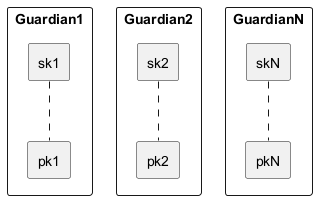
\includegraphics[width=\textwidth]{abbildungen/Diagramme/keyceremony1.png}
        \caption{Key generation}
        \label{fig:keypair}
    \end{subfigure}
    \hfill
    \begin{subfigure}{0.3\textwidth}
        \centering
        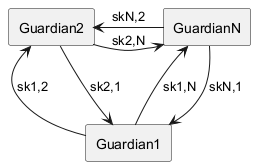
\includegraphics[width=\textwidth]{abbildungen/Diagramme/keyceremony2.png}
        \caption{Backup sharing}
        \label{fig:backup}
    \end{subfigure}
    \hfill
    \begin{subfigure}{0.3\textwidth}
        \centering
        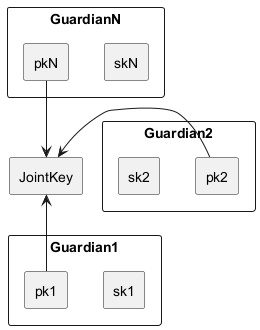
\includegraphics[width=\textwidth]{abbildungen/Diagramme/keyceremony3.png}
        \caption{Joint key generation}
        \label{fig:jointkey}
    \end{subfigure}
    \caption{Illustration of the Key Ceremony Process. Adapted from \cite{eg-docs}}
    \label{fig:keyceremony}
\end{figure}
The key-generation ceremony involves trustworthy individuals, known as \textbf{Guardians}, who collaborate to create a joint election key through the multiplication of individual public keys \cite{eg-docs}. The steps involved in the key-generation ceremony are illustrated in Figure \ref{fig:keyceremony}. The joint key is essential for encrypting data, as it requires all Guardians to apply their private keys for decryption. This process minimize the risk associated with a single party being responsible for the property of ballot confidentiality \cite[8]{eg-paper}. It is crucial to recognize that at least some level of trust is necessary for any component of the system. To ensure the distribution of trust is effective, it is essential that the Guardians are genuinely independent of each other \cite[92]{stuve-study}. If some Guardians are unavailable in the post-election phase the quorum count allows a specified number of Guardians to reconstruct missing private keys by sharing "backup" copies among themselves during the pre-election phase \cite[8]{eg-paper}  \cite{eg-docs}. The last step in the pre-election phase involves loading the election manifest, cryptographic parameters, and the joint key into an encryption device responsible for encrypting ballots throughout the intra-election phase. \cite[8]{eg-paper}.

\subsection{Intra-Election Ballot Encryption}
\begin{figure}[ht!]
    \centering
    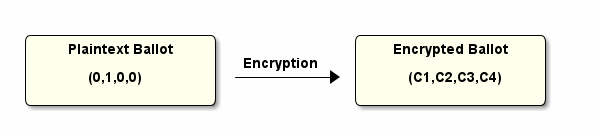
\includegraphics[scale=.5]{abbildungen/Diagramme/ballotencryption.png}
    \caption{Representation of Plaintext and Encrypted Ballots Adapted from \cite{eg-docs}} \label{Fig:ballot-representation}
\end{figure}
During the election phase, the ballots are encrypted and consist entirely of exponential ElGamal encryptions of binary values: a "1" signifies support for a particular option, while a "0" indicates a lack of support \cite[11]{eg-paper} \cite[12]{eg-spec}. In scenarios where a voter has multiple options, such as four choices in a single contest, the encrypted ballot will contain four corresponding encrypted bits. The exponential form of ElGamal encryption possesses an additive homomorphic property; therefore, the product of the encryption reflects the count of selected options \cite[5]{eg-spec}. A simple representation of this scenario is shown in Figure \ref{Fig:ballot-representation}. The plaintext ballot consists of four options in which the second option has been selected. When all encrypted values are combined homomorphically by multiplying them, the result encrypts the count of selections made. This technique ensures that the ballot does not contain excessive votes \cite[5]{eg-spec}.

While encryption itself is a straightforward process, a significant portion of ElectionGuard's effort is dedicated to creating externally verifiable artifacts to confirm that each encryption is well-formed \cite[3]{eg-spec}. \ac{ZK} proofs are employed to validate that the encryptions correspond to the values of 1 or 0 \cite[11]{eg-paper}. A Chaum-Pedersen proof verifies whether an encryption represents a specific value. By utilizing the Cramer-Damgård-Schoenmakers technique, it can be demonstrated that an encryption belongs to a specific set of values, such as "0" or "1". The proofs are made non-interactive through the Fiat-Shamir heuristic \cite[6,13]{eg-spec}. Once the encryption of a ballot is finalized, a confirmation code is generated for the voter \cite[17]{eg-spec}. This confirmation code is a cryptographic hash derived entirely from the encrypted ballot \cite[14]{eg-paper}. With the confirmation code, a voter can either cast the associated ballot or choose to spoilt it and restart the ballot preparation process. The two choices are mutually exclusive, since challenging reveals the ballot selections during the decryption phase. A challenged ballot can never be cast, while a cast ballot cannot be challenged anymore. This casting and spoiling mechanism acts as an interactive proof to assure voters that their selections have been correctly encrypted \cite[17]{eg-spec} \cite{eg-docs}.

\subsection{Post-Election Decryption of Tallies}
At the end of the voting period, all encrypted ballots submitted for tallying are homomorphically combined to produce an encrypted tally \cite[5,18]{eg-spec} \cite[15]{eg-paper}. Each available Guardian utilizes their private key to generate a decryption share, which represents a partial decryption for the encrypted tally or spoiled ballots. Decrypting spoiled ballots is unnecessary for determining the election outcome but may be performed to support cast-as-intended verifiability \cite[15,17]{eg-paper} \cite[18]{eg-spec}. To verify the correctness of these shares, Guardians also publish a Chaum-Pedersen proofs for each share \cite[18]{eg-spec}. The full decryption is achieved through the ordinary multiplication of these partial decryptions. If any Guardians are unavailable during decryption, the remaining Guardians can utilize the backups to reconstruct the missing shares \cite{eg-docs}.

To conclude the election, the final step involves the publication of the election record, which is vital for the integrity of a verifiable election. This record contains a complete account of all election artifacts, including the election manifest, cryptographic parameters, and the decrypted tally \cite[24]{eg-spec}. Independent verification software can be leveraged at any time after completion of an election to confirm the election's integrity \cite[6]{eg-paper}. The true value of a verifiable election is fully realized only when the election is actively verified by voters, election obsevers, or news organisations \cite[17]{eg-spec}. 

\section{ESP32-WROOM-32 Overview}
The \textbf{ESP32-WROOM-32} is a powerful microcontroller module that integrates Wi-Fi, Bluetooth, and \ac{BLE} technologies, along with 4MB of integrated SPI flash memory. At the core of this module is the ESP32-D0WDQ6 chip, which belongs to the ESP32 series of chips  \cite[6]{esp32-module}. In the context of this thesis, the term \textbf{ESP32} broadly refers to the family of chips within the series rather than a specific variant. It's important to note that the ESP32-WROOM-32 module is marked as not recommended for new designs. Instead, designers are advised to use the ESP32-WROOM-32E, which is built around either the ESP32-D0WD-V3 or the ESP32-D0WDR2-V3 chips \cite[1]{esp32-module-new}. These later revisions rectify some hardware issues \cite[3-4]{esp32-errata} present in previous versions. The ESP32-D0WDQ6 chip is susceptible to fault injection attacks. Successfully carrying out a fault injection attack could enable an attacker to recover the Flash Encryption key. This key allows unauthorized access to the device's flash contents, including firmware and data stored in flash. Such an attack necessitates physical access to the device \cite{chip-revision}. 
\begin{figure}[ht!]
	\centering
	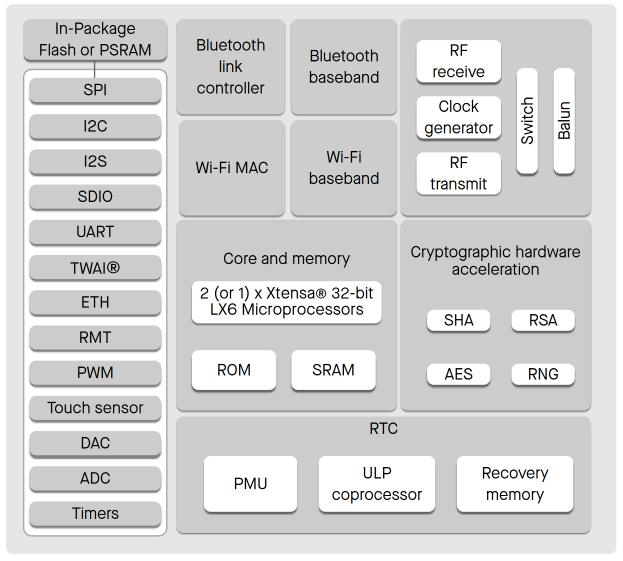
\includegraphics[scale=.5]{abbildungen/functional-block-diagram}
	\caption{ESP32 Functional Block Diagram} \label{Fig:esp32-crypto}
\end{figure}
ESP32 is designed for robustness, versatility, and reliability across a wide range of applications and power scenarios \cite[2]{esp32-series}. Due to its low power consumption, ESP32 is an ideal choice for \ac{IoT} applications spanning smart homes, industrial automation, consumer electronics, healthcare, and battery-powered electronics \cite[5]{esp32-series} \cite[6]{esp32-module}. ESP32 devices come with either a single or dual-core Xtensa® 32-bit LX6 microprocessor, operating at frequencies of up to 240 MHz. They come equipped with:
\begin{itemize}
    \item \textbf{448 KB of ROM} for booting and core functions \cite[4-5]{esp32-series}
    \item \textbf{520 KB of SRAM} for data and instructions \cite[4-5]{esp32-series}
    \item \textbf{34 programmable GPIOs} \cite[4-5]{esp32-series}
    \item \textbf{Cryptographic hardware acceleration capabilities} \cite[4-5]{esp32-series}
\end{itemize}

The supported cryptographic hardware acceleration capabilities include \ac{AES}, \ac{SHA}, \ac{RSA}, and \ac{RNG} \cite[4-5]{esp32-series}. A functional block diagram illustrating the components and subsystems within ESP32 is presented in Figure \ref{Fig:esp32-crypto}.

\subsection{Development Environment}
\begin{figure}[ht!]
	\centering
	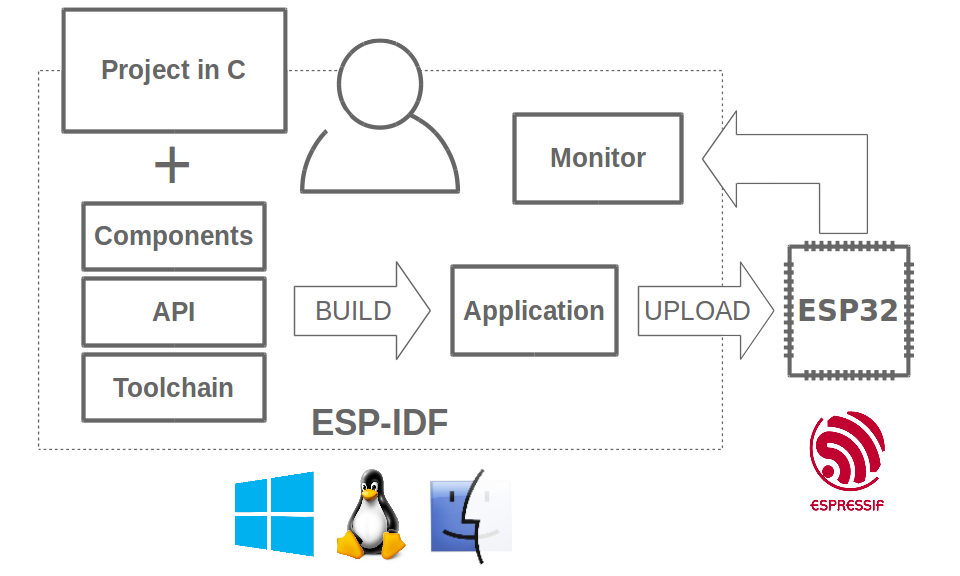
\includegraphics[scale=.5]{abbildungen/esp-idf.png}
	\caption{\ac{ESP-IDF} \cite[2805]{esp-prog}} \label{Fig:esp-idf}
\end{figure}
For application development, Espressif, the company behind the ESP32, offers the \ac{ESP-IDF}. \ac{ESP-IDF} encompasses a comprehensive toolchain, API components, and defined workflows tailored for ESP32 application development \cite[14]{esp-prog}. The development workflow for \ac{ESP-IDF} is depicted in Figure \ref{Fig:esp-idf}. \ac{ESP-IDF} consists of components written specifically for \ac{ESP-IDF} as well as third-party libraries \cite[2801]{esp-prog}. For example, the real-time operating system kernel used for \ac{ESP-IDF} applications is the third-party component called FreeRTOS \cite[2412]{esp-prog} \cite[6]{esp32-module}. \ac{ESP-IDF} projects use the same component based approach and can be seen as an amalgamation of a number of components. Components are modular pieces of standalone code that are compiled into static libraries which are subsequently linked into a project. These components can originate from various sources, including external git repositories or Espressif's Component Manager. Each component may also come with a Kconfig file, allowing users to configure the component through a text-based menu system \cite[2412-2413]{esp-prog}   


